\documentclass[conference]{IEEEtran}
\usepackage[T1]{fontenc}
\usepackage{amsmath,amssymb}
\usepackage{graphicx}
\usepackage{xcolor}
\usepackage{tikz}
\usetikzlibrary{shapes.geometric,arrows.meta,positioning,fit}
\usepackage{booktabs}
\usepackage{url}
\newcommand{\code}[1]{\texttt{#1}}

\begin{document}

\title{Vehicle Classification, Tracking and Counting on a Grid-Based
Motion-Detection Baseline: Verified-Equivalent Sequential and Parallel
Implementations and What Threading Actually Buys}

\author{
\IEEEauthorblockN{Jay Suriya R}
\IEEEauthorblockA{Department of Computer Science and Engineering\\
Indian Institute of Information Technology Sri City\\
Sri City, India\\
jaysuriya.r24@iiits.in}
\and
\IEEEauthorblockN{Manipriya Sankaranarayanan}
\IEEEauthorblockA{Department of Computer Science and Engineering\\
Indian Institute of Information Technology Sri City\\
Sri City, India\\
manipriya.s@iiits.in}
}

\maketitle

\begin{abstract}
A published grid-based (``virtual lattice'') vehicle detector marks each
cell of a region of interest (ROI) as moving or static and dispatches
the per-cell work to a thread pool, but its released implementation stops
at a binary occupancy grid. We build on its front end a rule-based
vehicle classifier, multi-object tracking with line-crossing counting,
adaptive density estimation and calibration-based speed estimation (implemented
but not validated), in a sequential implementation and a two-lane parallel
implementation with persistent thread pools and per-lane state. A cross-implementation check
on UA-DETRAC found two preprocessing divergences between the supposedly
identical implementations; after fixing them, both produce matching confusion
matrices and F1 scores on all 12 test videos. A grid-resolution study with
site-grouped cross-validation, trajectory-based counting ground truth and
44 unseen-site test videos shows that, once thresholds are re-tuned per
grid, finer lattices bring no significant classification gain, while the
finest one ($10{\times}12$) over-counts markedly. We then time four
workloads that separate lane count from threading on a 4-core/8-thread
CPU. Threading does \emph{not} reduce execution time: the threaded
two-lane run is slower than the same code without threads (time ratio
$0.860\pm0.077$, slower on all 12 videos). The two-lane implementation's
$1.26\times$ higher ROI-frame throughput over the one-lane script comes
from sharing per-frame decoding and preprocessing between lanes
(unthreaded: $1.46\times$), and the single-threaded script already keeps
about four cores busy through OpenCV's internal threading. The results
show that ``same algorithm, parallelized'' and ``parallel is faster''
must be measured with matched workloads rather than assumed.
\end{abstract}

\begin{IEEEkeywords}
vehicle classification, multi-object tracking, vehicle counting,
parallel computing, thread pool, Python GIL, benchmarking, UA-DETRAC
\end{IEEEkeywords}

\section{Introduction}
\label{sec:intro}
Existing road cameras can support vision-based vehicle counting and
classification without inductive loops or radar \cite{crouzil2016}.
Recent systems combine learned detectors with multi-object trackers,
e.g.\ YOLOv7 with DeepSORT \cite{lian2025} or an improved YOLOv8 with
BoT-SORT \cite{liu2025}; model size, power and throughput are recognized
obstacles on edge hardware \cite{zhai2023}, which lightweight
architectures and quantization reduce \cite{chang2025,macko2025}.
Classical foreground-segmentation pipelines remain a training-free
alternative for counting and coarse classification \cite{unzueta2012},
although illumination changes, shadows and occlusion make them fragile
\cite{abbas2021,chen2020}.

Two-Tier Parallel Virtual Lattice Layers (TPL2) \cite{baseline} divides
each lane's ROI into a grid, marks cells by histogram-equalized frame
differencing and per-cell contour detection, and dispatches cells and
lanes to a \code{ThreadPoolExecutor}. The TPL2 paper describes a
lattice-run counting heuristic and count-based density, leaves speed
estimation to future work, and reports execution time and memory
(26.55\% efficiency gain, 3.72\% more memory) but no accuracy metrics
\cite{baseline,muthuraja2026}. Its released code, which we build on,
stops at the occupancy grid and creates a new thread pool every frame
without persistent per-lane state (Table~\ref{tab:baseline}).

We contribute: (1) a classification, tracking, counting and
adaptive-density layer on that front end, with a calibration-based speed
estimator whose accuracy is not validated here, implemented identically in
a sequential (\code{seq.py}) and a two-lane parallel
(\code{rparallel\_he3.py}) implementation; (2) a parallel design with
persistent pools, per-lane \code{LaneTracker} state and a compute/draw
split; (3) a UA-DETRAC evaluation at grid and vehicle level;
(4) a cross-implementation check that found and fixed two preprocessing
divergences; (5) a four-workload benchmark that separates the effect
of processing two lanes from the effect of threading, showing that the
threads do not reduce execution time on the evaluated machine; and (6) a
grid-resolution study with site-grouped cross-validation, counting ground
truth from annotated trajectories and an unseen-site test set.

\begin{table}[t]
\centering
\caption{Baseline \cite{baseline} vs.\ this paper.}
\label{tab:baseline}
\scriptsize
\setlength{\tabcolsep}{3pt}
\begin{tabular}{p{3.85cm}p{4.2cm}}
\toprule
\textbf{Baseline (paper / released code)} & \textbf{This paper} \\
\midrule
ROI grid; HE frame differencing; per-cell contours & reused; retuned parameters; two divergences fixed \\
-- & geometric vehicle classification \\
lattice-run count heuristic (paper) & tracking, duplicate suppression, line-crossing counts \\
speed left to future work & displacement-gated speed estimation \\
raw occupancy (code), count-based density (paper) & adaptive thresholds with flow blending \\
pool created per frame, no per-lane state & persistent pools, per-lane \code{LaneTracker} \\
time and memory only & UA-DETRAC accuracy; four-workload timing \\
\bottomrule
\end{tabular}
\end{table}

\section{Related Work}
\label{sec:related}
Frame differencing and background subtraction remain competitive with
more elaborate background models in urban traffic video at a fraction of
the cost \cite{cheung2004}, and support real-time counting and
classification \cite{unzueta2012,crouzil2016}. A contemporaneous
extension of the same baseline \cite{muthuraja2026} adds scene-adaptive
preprocessing (illumination classes, CLAHE, a Dark Channel Prior fog
index) and reaches 71.03\% micro-averaged F1 on 60 UA-DETRAC sequences
with Hungarian matching; its multi-\emph{process} engine reaches
$1.34\times$ over sequential execution, with inter-process serialization
and sequential tracking identified as the binding constraints. That
pipeline differs from ours, so its process-level result and our
thread-level result are not directly comparable. SORT \cite{bewley2016} and DeepSORT \cite{wojke2017}
are standard tracking alternatives to our greedy association.
Pixel-displacement speeds need a metric scale and validation against
measured speeds \cite{kamil2024}, and unstable trajectories degrade them
\cite{sangsuwan2024}. Contours follow Suzuki and Abe's border following
\cite{suzuki1985}; data come from UA-DETRAC \cite{wen2020}. CPython's GIL
serializes bytecode across threads \cite{pythongil}, but
\code{ThreadPoolExecutor} \cite{pythonfutures} can overlap native calls
that release it. Amdahl's law \cite{amdahl1967,alhayanni2020},
\begin{equation}
S(N)=\frac{1}{(1-p)+p/N},
\label{eq:amdahl}
\end{equation}
bounds the speedup for parallel fraction $p$ on $N$ workers; a
single-fraction model cannot capture contention between resources
\cite{poolla2023}. We follow reporting recommendations for reliable
benchmarking \cite{beyer2019,kalibera2013}.

\section{Methodology}
\label{sec:method}

\subsection{Pipeline Overview}
Fig.~\ref{fig:roi} shows the two ROIs and Fig.~\ref{fig:pipeline} the
per-ROI pipeline. The sequential implementation (\code{seq.py})
processes ROI~1; the two-lane parallel implementation processes ROI~1 and
ROI~2 as independent lanes. Fig.~\ref{fig:stages}
shows the intermediate results of one frame, and Fig.~\ref{fig:overlay}
the annotated output of the two-lane parallel implementation.

\begin{figure}[t]
\centering
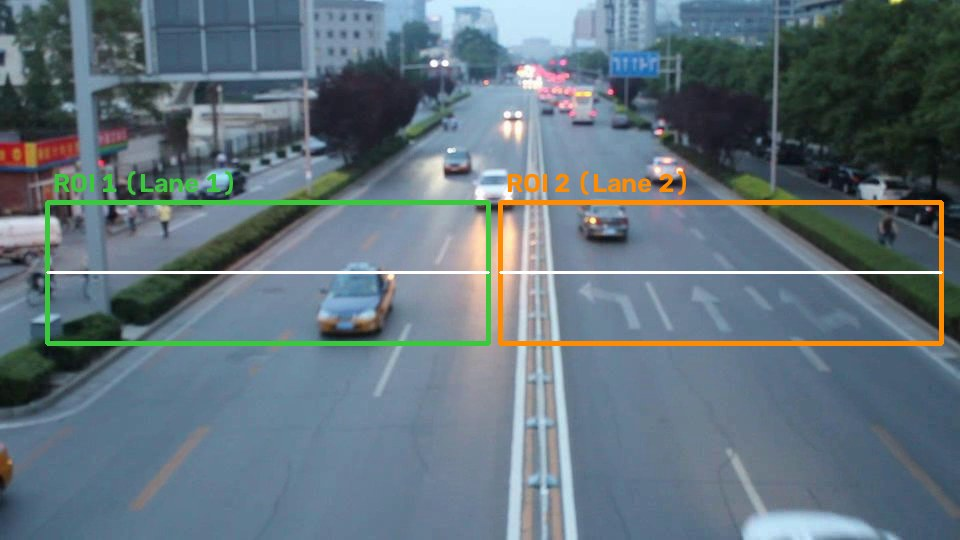
\includegraphics[width=\columnwidth]{figures/fig_roi_frame.jpg}
\caption{UA-DETRAC frame (MVI\_39761) with ROI~1 (green, Lane~1) and
ROI~2 (orange, Lane~2); white lines are the count lines.}
\label{fig:roi}
\end{figure}

\begin{figure*}[t]
\centering
\resizebox{\textwidth}{!}{%
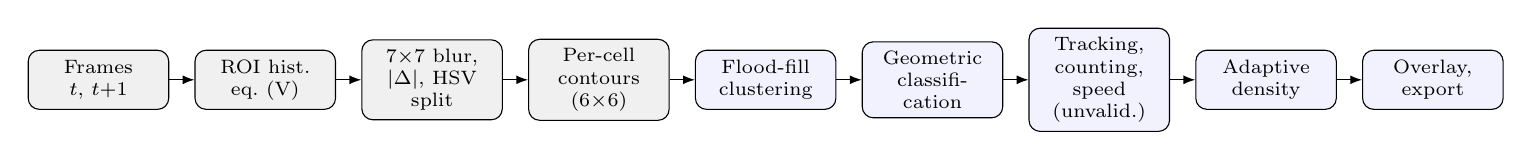
\begin{tikzpicture}[
  box/.style={draw, rounded corners, align=center, minimum height=0.75cm,
              text width=1.55cm, font=\scriptsize, fill=blue!5},
  base/.style={box, fill=gray!12},
  arr/.style={-{Latex[length=1.5mm]}}, node distance=3.2mm]
\node[base] (a) {Frames $t$, $t{+}1$};
\node[base, right=of a] (b) {ROI hist.\ eq.\ (V)};
\node[base, right=of b] (c) {$7{\times}7$ blur, $|\Delta|$, HSV split};
\node[base, right=of c] (d) {Per-cell contours ($6{\times}6$)};
\node[box, right=of d] (e) {Flood-fill clustering};
\node[box, right=of e] (f) {Geometric classification};
\node[box, right=of f] (g) {Tracking, counting, speed (unvalid.)};
\node[box, right=of g] (h) {Adaptive density};
\node[box, right=of h] (i) {Overlay, export};
\foreach \x/\y in {a/b,b/c,c/d,d/e,e/f,f/g,g/h,h/i} \draw[arr] (\x) -- (\y);
\end{tikzpicture}%
}
\caption{Per-ROI pipeline. Gray: baseline front end (reused, retuned);
blue: added in this work.}
\label{fig:pipeline}
\end{figure*}

\begin{figure*}[t]
\centering
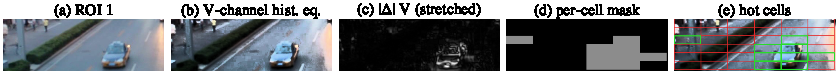
\includegraphics[width=\textwidth]{figures/fig_stages.pdf}
\caption{Processing stages for ROI~1 (MVI\_39761, frame 700): (a) input,
(b) V-channel histogram equalization, (c) absolute difference of the
blurred frames, V channel (contrast-stretched for display), (d) per-cell
thresholded and dilated masks, (e) cells with a valid contour (green).}
\label{fig:stages}
\end{figure*}

\subsection{Grid-Based Motion Detection (Baseline Front End)}
\label{sec:motion}
Both frames are histogram-equalized on the ROI's V channel (the
equalization channel is fixed to V), blurred with a $7\times7$ Gaussian
and differenced; the difference is converted to HSV and the configured
channel (V) is split out. Each cell is blurred ($5\times5$, $\sigma{=}1$),
thresholded at 60, dilated with a (cell width, cell height/2) rectangle
for 5 iterations, and marked ``hot'' if \code{cv2.findContours}
(\code{RETR\_EXTERNAL}) returns a contour larger than 100\,px$^2$ (AND
across channels if several are selected). Relative to the baseline we
retuned the threshold ($20\to60$), dilation (fixed kernel, 3
iterations $\to$ cell-sized, 5), retrieval mode (\code{RETR\_TREE} $\to$
\code{RETR\_EXTERNAL}) and blur $\sigma$ ($0\to1$), because the classifier
depends on precise cluster spans. Table~\ref{tab:params} lists all
constants.

\begin{table}[t]
\centering
\caption{Pipeline parameters (identical in both implementations).}
\label{tab:params}
\scriptsize
\setlength{\tabcolsep}{3pt}
\begin{tabular}{ll}
\toprule
ROI 1 / ROI 2 $(x,y,w,h)$ & (47,202,441,141) / (500,202,441,141) \\
Grid; cell blur / threshold & $6\times6$; $5\times5$ Gaussian / 60 \\
Dilation; min.\ contour area & (cell$_w$, cell$_h$/2), 5 iters; 100 px$^2$ \\
Track match radius; dup.\ IoU & ROI height/2; 0.40 \\
Crossing cooldown; eviction & 30 frames, 60 px; unseen $>2$\,s \\
Label EWA $\alpha$; min.\ frames scored & 0.15; 5 \\
Speed gate; smoothing & 3$\times$cell height; last 15 samples \\
Density blend; flow norm. & 0.7/0.3; 8 crossings per 2\,s \\
Density thresholds & 0.30/0.60, then 0.25/0.55 $\pm$0.10 adaptive \\
\code{\_CELL\_POOL} / \code{\_LANE\_POOL} & $\min(32,4{\times}\text{cpu})$ = 32 / 2 \\
\bottomrule
\end{tabular}
\end{table}

\subsection{Clustering and Classification}
\label{sec:classify}
Hot cells are grouped into objects by 4-connected flood fill; each
cluster gets a bounding box, centroid and the number of distinct columns
and rows it spans. With spans normalized by the grid size, a cluster is
a \textbf{Bus} if its column span exceeds 0.75 or both spans exceed
0.55, a \textbf{Van} if its row span exceeds 0.45, and a \textbf{Car}
otherwise. No appearance features are used, so the thresholds are tied
to this camera geometry. Their dependence on the lattice resolution is
examined in Section~\ref{sec:grid-sensitivity}.

\subsection{Tracking, Counting and Density}
\label{sec:tracking}
Objects are greedily matched to tracks by nearest centroid within half
the ROI height, one object per track; unmatched objects open tracks.
Each track accumulates classifications weighted by
$(cy/H)\,(1{+}\alpha)^{\text{age}}$, and its label enters evaluation once
it is at least 5 frames old. Of two tracks with IoU $>0.40$, the younger
is suppressed. A crossing is counted when the centroid passes the ROI's
mid-line (track age $\geq 2$), unless it lies within 30 frames and 60\,px
of a previous crossing. Density blends the smoothed hot-cell fraction
(0.7) with recent flow (0.3); Low/Medium/High thresholds adapt to the
33rd/66th percentiles of the history within $\pm0.10$ of their base
values.

\subsection{Speed Estimation (Implemented, Not Validated)}
\label{sec:speed}
The image-to-metric scale is calibrated from two points that span a
known real-world distance in the video, such as a lane width, a lane-mark
period or a vehicle width (Fig.~\ref{fig:speed}a): with pixel distance
$d$ between the clicked points (converted from display to native video
coordinates) and real distance $L$, $k=d/L$ pixels per meter. A
command-line tool can average several such pairs and warns when their
coefficient of variation exceeds 15\%. For each track, centroid displacement is
accumulated until it reaches three cell heights, which suppresses grid
quantization; a speed sample is then
\begin{equation}
v=\frac{\Delta d_{\text{px}}/k}{\Delta n/f}\times3.6\ \text{km/h},
\label{eq:speed}
\end{equation}
where $\Delta n$ frames have elapsed at frame rate $f$, and the displayed
speed is the moving average of the track's last 15 samples
(Fig.~\ref{fig:speed}b). A single scale $k$ ignores perspective
foreshortening along the road. \textbf{No speed accuracy is claimed}: no
speed ground truth exists for the test videos, and $k=0$ in all benchmark
runs, which disables the computation. In a qualitative calibrated run
the overlay showed plausible values (e.g.\ 42--43\,km/h) next to
implausible ones (above 400\,km/h for some tracks), as expected when
cluster centroids jump between frames; validation against measured
speeds and perspective-correct scaling are required
\cite{kamil2024,sangsuwan2024}.

\begin{figure*}[t]
\centering
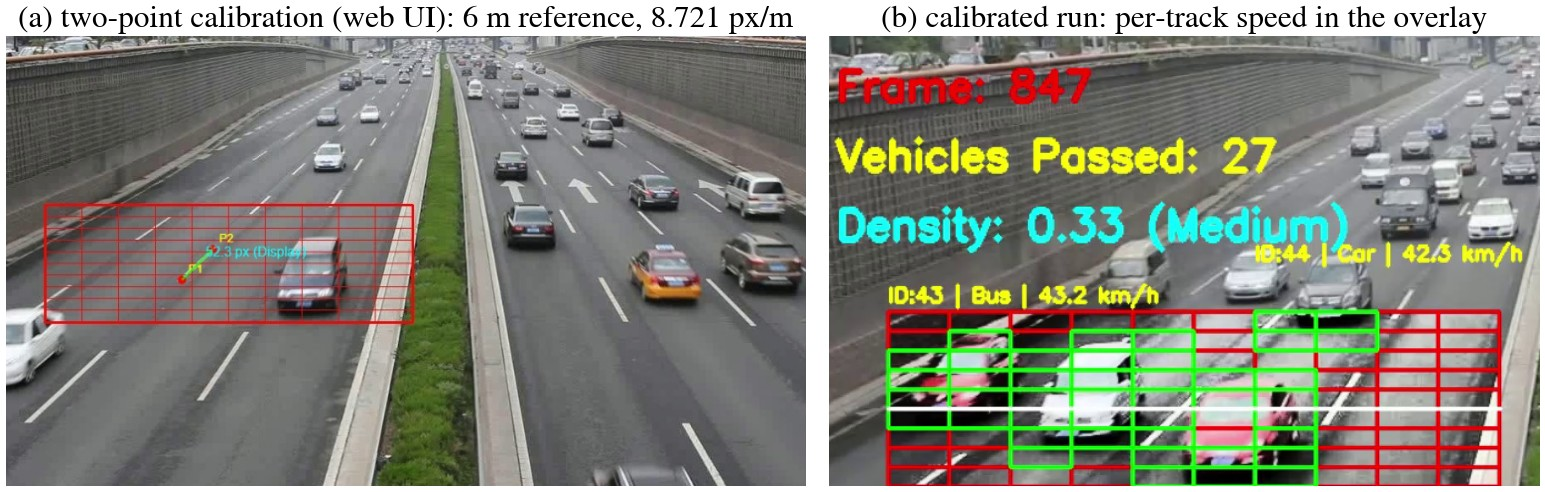
\includegraphics[width=0.92\textwidth]{figures/fig_speed.jpg}
\caption{Speed-estimation module (not part of the benchmark): (a)
two-point calibration in the web interface, here a 6\,m reference
giving 8.721\,px/m; (b) a frame of a calibrated qualitative run with
per-track speeds in the overlay (finer grid than in the benchmark).
The speeds are unvalidated; other frames of the same run show
implausible values.}
\label{fig:speed}
\end{figure*}

\subsection{Parallel Implementation}
\label{sec:parallel}
Two persistent pools are created once (Fig.~\ref{fig:threadpools}):
\code{\_CELL\_POOL} runs per-cell contour extraction (\code{map}) and the
per-ROI equalization (\code{submit} from the main thread), and
\code{\_LANE\_POOL} (2 workers) runs each lane's grid detection and
tracking update. Keeping the pools separate prevents a lane task from
waiting on a worker slot in its own pool. All mutable per-lane state
lives in a \code{LaneTracker} instance, so concurrent lane updates touch
disjoint memory; drawing on the shared frame happens serially, Lane~1
then Lane~2, after both updates finish. The full-frame blur, difference
and channel split run serially on the main thread.

\begin{figure}[t]
\centering
\resizebox{0.97\columnwidth}{!}{%
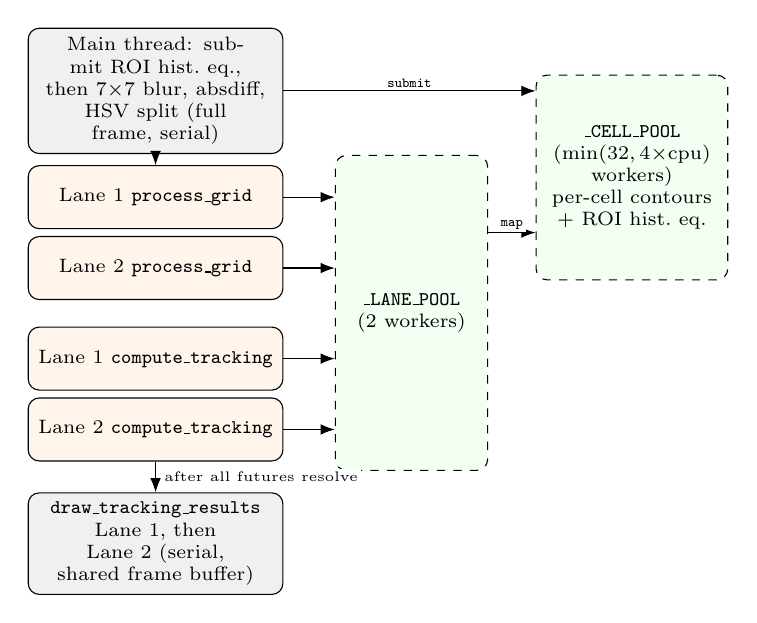
\begin{tikzpicture}[
  box/.style={draw, rounded corners, align=center, minimum height=0.8cm,
              text width=3.0cm, font=\scriptsize, fill=orange!8},
  serial/.style={box, fill=gray!12},
  pool/.style={draw, dashed, rounded corners, align=center, font=\scriptsize,
               fill=green!5, text width=1.7cm},
  arr/.style={-{Latex[length=1.8mm]}},
  lbl/.style={font=\tiny, fill=white, inner sep=1pt}
]
\node[serial] (pre)   at (0, 0)    {Main thread: submit ROI hist.\ eq.,\\then $7{\times}7$ blur, absdiff,\\HSV split (full frame, serial)};
\node[box]    (l1)    at (0,-1.35) {Lane 1 \code{process\_grid}};
\node[box]    (l2)    at (0,-2.25) {Lane 2 \code{process\_grid}};
\node[box]    (t1)    at (0,-3.40) {Lane 1 \code{compute\_tracking}};
\node[box]    (t2)    at (0,-4.30) {Lane 2 \code{compute\_tracking}};
\node[serial] (draw)  at (0,-5.75) {\code{draw\_tracking\_results}\\Lane 1, then Lane 2 (serial,\\shared frame buffer)};
\node[pool, minimum height=4.0cm] (lanepool) at (3.25,-2.82) {\code{\_LANE\_POOL}\\(2 workers)};
\node[pool, minimum height=2.6cm, text width=2.2cm] (cellpool) at (6.05,-1.10) {\code{\_CELL\_POOL}\\($\min(32,4{\times}\text{cpu})$\\workers)\\per-cell contours\\+ ROI hist.\ eq.};
\foreach \n in {l1,l2,t1,t2} \draw[arr] (\n.east) -- (\n.east -| lanepool.west);
\draw[arr] (pre.east) -- node[lbl, above]{\code{submit}} (pre.east -| cellpool.west);
\draw[arr] (lanepool.east |- l1.east) ++(0,-0.45) coordinate (a) -- node[lbl, above]{\code{map}} (a -| cellpool.west);
\draw[arr] (pre.south) -- (l1.north);
\draw[arr] (t2.south) -- node[lbl, right, xshift=2pt]{after all futures resolve} (draw.north);
\end{tikzpicture}%
}
\caption{Per-frame dispatch in the two-lane parallel implementation.}
\label{fig:threadpools}
\end{figure}

\begin{figure}[t]
\centering
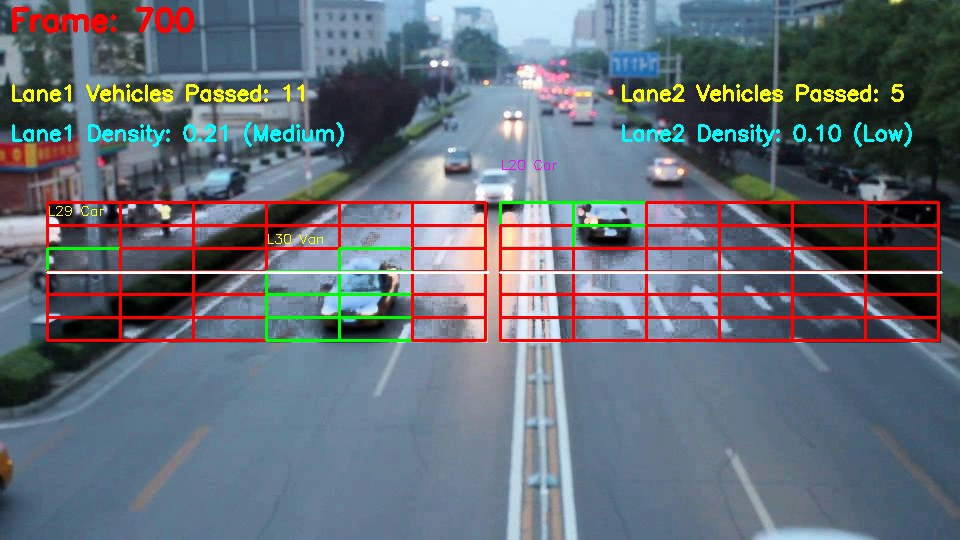
\includegraphics[width=\columnwidth]{figures/fig_overlay.jpg}
\caption{Output of the two-lane parallel implementation in the
benchmark run (MVI\_39761, frame 700): green cells are hot cells, labeled
boxes are tracks, white lines are count lines; per-lane counts and
density states are shown at top.}
\label{fig:overlay}
\end{figure}

\subsection{Evaluation}
\label{sec:eval}
UA-DETRAC XML boxes overlapping the ROI are mapped to \{Car, Van, Bus,
Unknown\}. At grid level, each box center labels a cell, giving a
$4\times4$ confusion matrix over \{Empty, Car, Van, Bus\}. At vehicle
level, each scored track is matched to the highest-IoU box ($>0.1$); the
majority label per ground-truth ID fills a $3\times3$ Car/Van/Bus matrix,
from which precision, recall and F1 are computed with a small
$\epsilon$. Predictions at frame $t$ are compared with ground truth at
$t{+}1$, ``others'' matched to a track count as Car, ignored regions are
not masked, and matching is greedy; these choices affect both implementations
equally.

\section{Experimental Setup}
\label{sec:experiments}
\textbf{Platform.} AMD Ryzen 5 7235HS laptop (4 cores, 8 logical
processors), Windows 11, Python 3.12.3, OpenCV 4.12.0, NumPy 1.26.4;
each metrics file records these values \cite{beyer2019}.

\textbf{Videos.} From each UA-DETRAC weather folder (Cloudy, Night,
Rainy, Sunny) we split the annotated videos into density terciles (mean
annotated vehicles per frame) and took the middle-ranked video of each,
giving 12 videos (2.81--14.92 vehicles/frame; 960$\times$540, 25\,fps;
14{,}356 frame pairs). Tiers are relative within each category; the
candidate pools were small (4/6/5/23 videos). Grid $6\times6$, channel V,
display and frame dumps disabled.

\textbf{Four workloads.} The sequential implementation processes one
ROI and the two-lane parallel implementation two, so their raw times are
not comparable. We therefore time: \textbf{A}~\code{seq.py} (1 lane);
\textbf{B}~the parallel implementation with Lane~1 only (threaded);
\textbf{C}~both lanes with the thread pools replaced by an inline executor
(same \code{LaneTracker} code and call order, no threads: the unthreaded
workload); and \textbf{D}~the parallel implementation (2 lanes, threaded). With end-to-end time $T$ and mean per-frame
processing time $\bar t$ (processing and drawing, excluding output I/O,
same boundaries in all workloads) we report per video
$S_{\text{naive}}=T_A/T_D$ (context only), the ROI-frame throughput ratio
$S_{\text{norm}}=2T_A/T_D$, its unthreaded counterpart
$S_{\text{amort}}=2T_A/T_C$, and the threads-only ratios
$S_{\text{same}}^{(2)}=T_C/T_D$ and $S_{\text{same}}^{(1)}=T_A/T_B$.
Because decoding, writing and the full-frame preprocessing are done once
per frame, $S_{\text{norm}}$ can exceed 1 without any benefit from
threading. Values are mean $\pm$ sample std over the 12 videos, i.e.\
between-video variation. Each workload ran once per video with the
profiler off; A and D were also run under \code{cProfile}. All numbers
are computed by \code{benchmarking/orchestrate\_benchmark.py}.

\section{Results and Discussion}
\label{sec:results}

\subsection{Accuracy and Cross-Implementation Equivalence}
\label{sec:crosscheck}
Because \code{seq.py} and Lane~1 of the parallel implementation run the
same deterministic logic on the same ROI, their confusion matrices should
agree exactly. Initially only 4 of 12 videos matched. The parallel
version lacked the $7\times7$ pre-difference blur; adding it raised the
match rate only to 5/12. The remaining divergence was in the
equalization itself: the parallel helper ignored the channel setting and
grayscaled the ROI, discarding hue and saturation, whereas \code{seq.py}
equalizes only V. (The pre-fix runs were not archived; both match rates
are taken from development logs.) After both fixes, Lane~1 of
workloads B, C and D matches \code{seq.py} on all 12 videos
(vehicle and grid matrices, ID counts and per-class P/R/F1, compared
exactly), and Lane~2 matches between C and D: 60/60 checks, including the
profiled pass. This shows agreement on the tested videos under this
protocol, not equivalence for every input.

\begin{figure}[t]
\centering
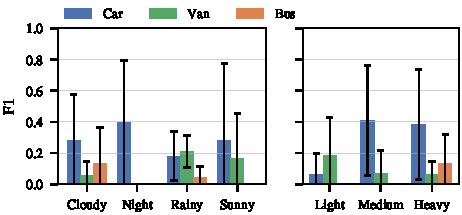
\includegraphics[width=\columnwidth]{figures/fig_f1.pdf}
\caption{Vehicle-level F1 (identical for all implementations), mean
$\pm$ std by weather category (3 videos each) and density tier (4
each).}
\label{fig:f1}
\end{figure}

Fig.~\ref{fig:f1} and Table~\ref{tab:prf} report the resulting
vehicle-level metrics, computed per video and averaged as elsewhere in
the paper. Accuracy is low and varies strongly between videos. Pooled
over the 12 videos, 179 of the 203 matched ground-truth vehicles are
cars, but the classifier labels 127 of them as vans; this systematic
Car$\to$Van bias of the fixed geometric thresholds explains the low Car
recall and the low Van precision. Vans and buses occur in the matched
ground truth of only 7 and 5 videos, and a class that is absent or never
reaches the minimum track age scores 0 for that video, so Bus F1 is 0 in
10 of 12 videos and in four of seven groups. The contribution of this
section is the verified agreement between implementations, not the
classifier's accuracy.

\begin{table}[t]
\centering
\caption{Vehicle-level precision, recall and F1 (identical for both
implementations), mean $\pm$ std over 12 videos.}
\label{tab:prf}
\scriptsize
\setlength{\tabcolsep}{4pt}
\begin{tabular}{lcccc}
\toprule
\textbf{Class} & \textbf{Precision} & \textbf{Recall} & \textbf{F1} & \textbf{Videos with class$^{a}$} \\
\midrule
Car & $0.51\pm0.46$ & $0.24\pm0.32$ & $0.29\pm0.31$ & 12 \\
Van & $0.07\pm0.11$ & $0.33\pm0.45$ & $0.11\pm0.16$ & 7 \\
Bus & $0.03\pm0.08$ & $0.10\pm0.23$ & $0.04\pm0.12$ & 5 \\
\bottomrule
\end{tabular}

\smallskip
\parbox{\columnwidth}{\scriptsize $^{a}$Videos whose matched ground truth
contains the class; in the other videos the class scores 0.}
\end{table}

\subsection{Grid Resolution Sensitivity and Its Impact on Vehicle Classification and Counting}
\label{sec:grid-sensitivity}
The lattice resolution fixes the cell size from which motion, object
extent and the span-based label are derived. We therefore compared six
resolutions ($4{\times}6$, $6{\times}6$, $6{\times}8$, $8{\times}8$,
$8{\times}10$, $10{\times}12$, rows$\times$columns) on the unthreaded
two-lane workload~C, with the pipeline otherwise unchanged.

\textbf{Protocol.} UA-DETRAC provides no camera-site labels. We therefore
grouped the 26 other annotated videos of the four weather folders into 10
sites by inspecting their static backgrounds. Using only these videos, the
grid and the classification thresholds were chosen by leave-one-site-out
cross-validation. In each fold, the thresholds were tuned per grid on the
training sites (810 candidates), and the grid was selected by a predefined
objective. The objective combines macro-F1, the weakest class F1, counting
event-F1, detection recall, fragmentation and unmatched detections, subject
to a real-time throughput guard. The resulting configuration was frozen
before testing. The test set consists of 44 further UA-DETRAC videos
(67{,}206 frames, 25 recording sessions). These videos were not used
elsewhere in this work, and their scenes differ from all tuning and
benchmark sites. The 12 benchmark videos of this paper share sites with
the tuning videos and had informed an earlier exploratory grid analysis,
so their grid results are not used for this comparison. Counting was
scored against line-crossing events extracted from the annotated
trajectories. Events were matched one-to-one within 1\,s and 80\,px. In
the combined two-lane score, both lanes compete for the same ground-truth
events, so a vehicle cannot be credited twice. The counter's events were
replayed from per-frame logs and reproduce its reported per-lane totals in
every run. These runs used a separate 2-vCPU Linux VM (OpenCV 5.0), so
their frame rates are not comparable with Section~\ref{sec:timing}.

\begin{figure}[t]
\centering
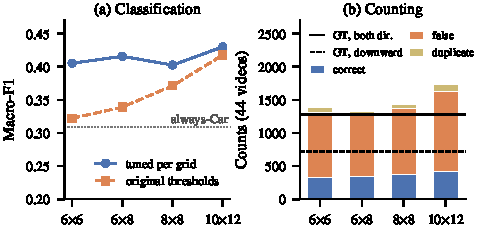
\includegraphics[width=\columnwidth]{figures/fig_grid.pdf}
\caption{Grid resolution on 44 unseen-site test videos. (a)~Vehicle-level
macro-F1 with the original thresholds and with thresholds tuned per grid
on the tuning videos. (b)~Combined-lane counts against trajectory
crossings: the counter registers only downward crossings.}
\label{fig:grid}
\end{figure}

\begin{table}[t]
\centering
\caption{Grid resolution on the 44 unseen-site test videos (frozen,
per-grid tuned thresholds; combined lanes). Count F1 and MAE (per video)
use downward trajectory crossings (720). FPS: median of 3 serial trials
on the VM.}
\label{tab:grid}
\scriptsize
\setlength{\tabcolsep}{3pt}
\begin{tabular}{lccccccc}
\toprule
\textbf{Grid} & \textbf{Macro-F1} & \textbf{Recall} & \textbf{Frag.} & \textbf{Counts} & \textbf{Count F1} & \textbf{MAE} & \textbf{FPS}\\
\midrule
$6{\times}6$   & 0.405 & 0.883 & 1.5\% & 1377 & 0.314 & 16.0 & 97.2\\
$6{\times}8^{a}$ & 0.416 & 0.892 & 2.3\% & 1318 & 0.336 & 14.9 & 91.9\\
$8{\times}8$   & 0.402 & 0.894 & 3.8\% & 1428 & 0.342 & 16.6 & 86.3\\
$10{\times}12$ & 0.430 & 0.908 & 9.5\% & 1728 & 0.337 & 23.1 & 81.4\\
\bottomrule
\end{tabular}

\smallskip
\parbox{\columnwidth}{\scriptsize $^{a}$Selected by site-grouped
cross-validation. Always-Car macro-F1: 0.31.}
\end{table}

\textbf{Classification.} With the original fixed thresholds, macro-F1
rose monotonically with resolution (Fig.~\ref{fig:grid}a). The
cross-validated value went from 0.12 at $4{\times}6$ to 0.31 at
$10{\times}12$. Once the thresholds were tuned per grid, the trend
vanished: cross-validated macro-F1 was 0.30--0.35 for every grid. On the
test set, no grid differed significantly from $6{\times}6$
(Table~\ref{tab:grid}; 95\% session-level paired bootstrap). The apparent
resolution effect is therefore mainly a calibration effect of the fixed
normalized-span thresholds. All tuned classifiers exceeded the always-Car
baseline on the test set (0.40--0.43 vs.\ 0.31), but Van F1 stayed at or
below 0.16.

\textbf{Counting.} Finer grids found slightly more vehicles (recall
0.883 to 0.908) and produced more correct counts (329 to 413). They also
produced more false and duplicate counts (Fig.~\ref{fig:grid}b). At
$10{\times}12$, the counter reported 1{,}728 crossings against 720
countable ones, and the per-video absolute error rose to 23.1, compared
with 14.9 at $6{\times}8$. Fragmentation grew from 1.5\% to 9.5\%. We
tested two diagnostic clustering variants, run separately from the
evaluated pipeline. Bridging a single empty cell row removed 87--89\% of
the fragmentation, and 8-connectivity removed 35--40\%. Fragmentation
thus comes mainly from vehicle interiors that frame differencing leaves
unmarked at small cell sizes. Neither variant improved classification.
Independently of resolution, the counter registers only downward
crossings, so it misses 44\% of the test crossings.

\textbf{Selected configuration.} The predefined rule selected
$6{\times}8$ with tuned thresholds. It was the only grid whose objective
improved significantly on $6{\times}6$ on the test set, at 92 vs.\
97\,FPS. Its margin over $8{\times}8$ and $10{\times}12$ lies within
fold-to-fold variation, so no resolution is universally best. Beyond
about $6{\times}8$, a finer lattice trades counting reliability for
classification gains that are small and not statistically supported. The
span features and the single-direction counter limit performance more
than the grid does. The benchmark experiments in this paper keep the
original $6{\times}6$ configuration.

\subsection{Timing: Four Workloads}
\label{sec:timing}

\begin{table}[t]
\centering
\caption{Four workloads (clean pass), mean $\pm$ std over 12 videos.}
\label{tab:timing}
\scriptsize
\setlength{\tabcolsep}{2.5pt}
\begin{tabular}{lcccccc}
\toprule
 & \textbf{Ln.} & \textbf{Loop (ms)} & \textbf{I/O (ms)} & \textbf{FPS} & \textbf{Peak MB} & \textbf{CPU} \\
\midrule
A & 1 & $9.41\pm1.84$ & $2.26\pm0.46$ & $81.1\pm15.7$ & $302.5\pm1.9$ & $4.20\pm0.61$ \\
B & 1 & $11.10\pm1.99$ & $2.19\pm0.43$ & $72.0\pm12.2$ & $306.4\pm1.8$ & $4.01\pm0.50$ \\
C & 2 & $14.54\pm2.59$ & $2.09\pm0.36$ & $58.2\pm9.6$ & $306.0\pm3.0$ & $4.52\pm0.47$ \\
D & 2 & $17.46\pm3.73$ & $2.27\pm0.39$ & $50.1\pm9.4$ & $310.0\pm3.1$ & $3.94\pm0.70$ \\
\bottomrule
\end{tabular}

\smallskip
\parbox{\columnwidth}{\scriptsize Loop: per-frame processing and drawing;
I/O: video write and next-frame decode; FPS: video frames per second of
end-to-end time; CPU: process CPU time / wall time (cores).}
\end{table}

\begin{figure}[t]
\centering
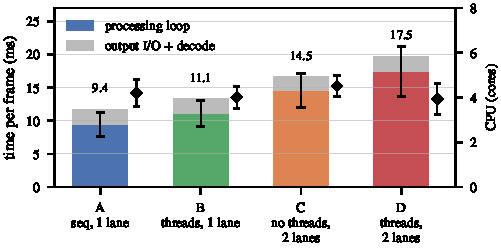
\includegraphics[width=\columnwidth]{figures/fig_workloads.pdf}
\caption{Per-frame time of the four workloads (bars, left axis) and CPU
use in cores (diamonds, right axis); mean $\pm$ std over 12 videos.}
\label{fig:workloads}
\end{figure}

Table~\ref{tab:timing} and Fig.~\ref{fig:workloads} summarize the
timings. Per video:
$S_{\text{naive}}=0.628\pm0.114$, $S_{\text{norm}}=1.257\pm0.228$
(per-frame loop: $1.097\pm0.187$), $S_{\text{amort}}=1.458\pm0.216$,
$S_{\text{same}}^{(2)}=0.860\pm0.077$ (loop: $0.842\pm0.081$) and
$S_{\text{same}}^{(1)}=0.900\pm0.123$. Three findings follow. First, the
two-lane parallel run takes longer than the one-lane sequential run on
every video. Second, \textbf{threading does not reduce execution time on
this machine}: with the workload fixed, the threaded run is slower than
the unthreaded one on all 12 videos with two lanes ($S_{\text{same}}^{(2)}$
0.69--0.93) and on 9 of 12 with one lane. Third, the normalized
throughput gain of D over A ($1.26$) is smaller than that of the
unthreaded run C over A ($1.46$), so it comes from processing two lanes
per decoded and preprocessed frame, not from threading
(Fig.~\ref{fig:ratios}). The threads-only efficiency
$E(N)=S_{\text{same}}^{(2)}/N$ is 0.43, 0.22 and 0.11 for $N=2,4,8$. The
threaded two-lane workload uses 7.5\,MB (2.5\%) more peak memory
than \code{seq.py}. An earlier run of A and D, with asymmetric timer
boundaries, gave $S_{\text{norm}}=1.261\pm0.084$ and identical accuracy.

\begin{figure}[t]
\centering
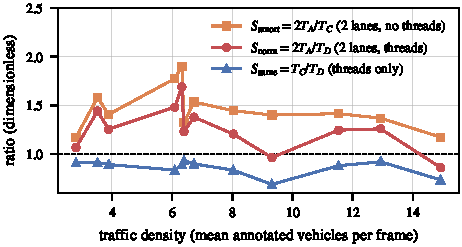
\includegraphics[width=\columnwidth]{figures/fig_ratios.pdf}
\caption{Per-video ratios against traffic density. Two lanes without
threads (C) gain more over the one-lane script than two lanes with
threads (D); threads alone ($T_C/T_D$) are below 1 on every video.}
\label{fig:ratios}
\end{figure}

$S_{\text{norm}}$ correlates weakly and negatively with density
(Pearson $r=-0.45$, $n=12$) and is lowest in the heavy tier
($1.08\pm0.20$ vs.\ $1.34$ light and $1.35$ medium). The cause is open:
the tracking stage takes only 1.6--4.2\% of sequential run time on every
video, with no density trend, and sequential loop time does not rise
with tier (11.4, 8.4, 8.4\,ms).

\subsection{Profiling and the Amdahl Ceiling}
\label{sec:results-amdahl}
In the sequential profile of the densest video (MVI\_39311, 1504
frames, 18.62\,s), the seven largest native OpenCV calls (\code{dilate},
\code{GaussianBlur}, \code{VideoCapture.read}, \code{cvtColor},
\code{absdiff}, \code{VideoWriter.write}, \code{split}) take 12.40\,s
(66.6\%), Python wrappers 0.99\,s, the main loop 1.62\,s, and the rest
3.61\,s (1.95\,s in further top-15 native calls such as
\code{findContours}, 0.51\,s). Counting only work reachable through
\code{\_CELL\_POOL} (per-cell contours and equalization) gives $p=0.362$
($0.375\pm0.019$ over all 12 videos); counting the seven native calls
gives $p=0.666$. At the lane-pool width $N=2$, Eq.~\eqref{eq:amdahl}
predicts 1.22 and 1.50 (Fig.~\ref{fig:amdahl}); the measured
threads-only ratio, 0.86, is below 1 and far from both. The narrow ceiling happens to lie close to $S_{\text{norm}}$ (1.22 vs.\
1.26), but the same-workload measurement shows that this proximity is
coincidental: $S_{\text{norm}}$ reflects shared per-frame work, not
threading.

\begin{figure}[t]
\centering
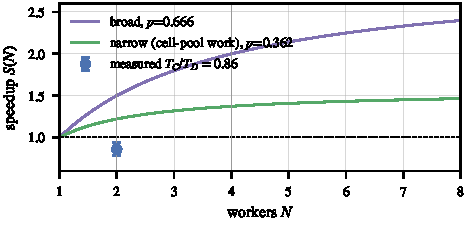
\includegraphics[width=\columnwidth]{figures/fig_amdahl.pdf}
\caption{Amdahl ceilings for the broad and narrow estimates of $p$
(MVI\_39311 profile) and the measured threads-only ratio $T_C/T_D$ at
$N=2$ (mean $\pm$ std).}
\label{fig:amdahl}
\end{figure}

\subsection{Why Threading Does Not Help Here}
\label{sec:why}
Three properties plausibly explain the result; only the first is
measured. (i) \textbf{The cores are already busy}: \code{seq.py} runs one
Python thread but uses $4.20\pm0.61$ cores (Table~\ref{tab:timing})
through native threads inside OpenCV, so Python-level threads compete
for occupied cores; CPU use does not rise with threading (3.94 cores for
D vs.\ 4.52 for C). (ii) \textbf{The tasks are small}: each frame
dispatches 36 tasks per lane on $73\times23$-pixel cells (\code{dilate}
averages $\approx$64\,$\mu$s per call), so dispatch overhead is a large
share of each task. (iii) \textbf{The GIL} serializes the Python parts
(wrappers, clustering, tracking). Separating (ii) and (iii) requires
further experiments, e.g.\ limiting OpenCV's internal threads or
batching cells. The baseline's 26.55\% gain \cite{baseline} was measured
with different code, configuration and hardware, so our results neither
reproduce nor contradict it.

\subsection{Threats to Validity}
\label{sec:threats}
All thresholds were tuned for one camera geometry, and illumination,
shadows and occlusion remain failure modes \cite{abbas2021,chen2020}.
Classification uses footprint geometry only and shows a systematic
Car$\to$Van bias. Speed estimation was not evaluated quantitatively, uses
a single scale without perspective correction, and produced implausible
values in a qualitative run (Section~\ref{sec:speed}).
Timings come from one laptop and one run per workload and video; the
reported spreads are between-video variation, and run-to-run variation is
visible (sequential loop $8.03\pm0.29$\,ms in the earlier run vs.\
$9.41\pm1.84$\,ms here). Repeated runs with confidence intervals
\cite{kalibera2013} and other machines are needed to bound noise, although
the threads-only result has the same sign on all 12 videos. An earlier
measurement suggesting about $3.3\times$ speedup was caused by an
unthrottled \code{cv2.waitKey} poll and a per-frame JPEG write in the
sequential script; both are now disabled in benchmarks, and the figure is
not used. Tracks younger than 5 frames are never scored, which excludes
short-lived vehicles from evaluation. The counter registers only downward crossings of
fixed ROIs, which misses traffic moving up the image (33--44\% of
annotated crossings in Section~\ref{sec:grid-sensitivity}). Camera sites
were inferred visually because UA-DETRAC has no site labels, and the
unseen-site test set still comes from the same dataset.

\section{Conclusion}
\label{sec:conclusion}
We added classification, tracking, counting and adaptive density
estimation, plus an unvalidated calibration-based speed estimator, to a
published grid-based detector, in a sequential and a two-lane parallel
implementation, and evaluated both on UA-DETRAC. A
cross-implementation check found and fixed two preprocessing divergences;
the implementations now agree exactly on all 12 test videos. A four-workload
benchmark on a 4-core/8-thread CPU showed that processing two lanes
raises ROI-frame throughput because decoding and preprocessing are shared
($1.46\times$ without threads, $1.26\times$ with threads), whereas the
thread pools themselves slow the same two-lane workload down
($0.86\times$), on a machine where the sequential script already uses
about four cores through OpenCV. A cross-validated grid-resolution study
with counting ground truth showed that finer lattices do not
significantly improve the re-tuned classifier and that the finest one
over-counts, so the span features and the single-direction counter, not
the grid, limit accuracy. Future work: direction-aware counting; limiting OpenCV's internal threading and
batching cells to test whether thread-level parallelism helps on idle
cores; a lightweight learned classifier \cite{chang2025,macko2025};
Kalman/Hungarian and appearance-based tracking \cite{bewley2016,wojke2017};
calibrated, validated speed estimation \cite{kamil2024}; and repeated-run
benchmarks on several machines. Code, data, metrics and figure scripts
are available in the project repository.


\begin{thebibliography}{99}

\bibitem{baseline}
M. Sankaranarayanan and K. SivaSai, ``Two-tier parallel virtual lattice
layers for enhanced efficiency in video traffic management,''
\emph{Int.\ J. Intell.\ Transp.\ Syst.\ Res.}, vol.~23, no.~1,
pp.~464--474, 2025, doi: 10.1007/s13177-025-00461-4.

\bibitem{muthuraja2026}
S. Muthuraja and M. Sankaranarayanan, ``Real-time traffic density
estimation using scene-adaptive parallel grid analysis,'' Research Square
preprint (in review), Jun.\ 2026, doi: 10.21203/rs.3.rs-9946108/v1.

\bibitem{crouzil2016}
A. Crouzil, L. Khoudour, P. Valiere, and D. N. Truong Cong, ``Automatic
vehicle counting system for traffic monitoring,'' \emph{J. Electron.\
Imaging}, vol.~25, no.~5, art.~051207, 2016, doi:
10.1117/1.JEI.25.5.051207.

\bibitem{lian2025}
H. Lian, M. Li, T. Li, Y. Zhang, Y. Shi, Y. Fan, W. Yang, H. Jiang,
P. Zhou, and H. Wu, ``Vehicle speed measurement method using monocular
cameras,'' \emph{Sci.\ Rep.}, vol.~15, art.~2755, 2025, doi:
10.1038/s41598-025-87077-6.

\bibitem{liu2025}
Y. Liu and S. Shen, ``Vehicle detection and tracking based on improved
YOLOv8,'' \emph{IEEE Access}, vol.~13, pp.~24793--24803, 2025, doi:
10.1109/ACCESS.2025.3538556.

\bibitem{zhai2023}
J. Zhai, B. Li, S. Lv, and Q. Zhou, ``FPGA-based vehicle detection and
tracking accelerator,'' \emph{Sensors}, vol.~23, no.~4, art.~2208, 2023,
doi: 10.3390/s23042208.

\bibitem{chang2025}
L. Chang, Q. Tang, J. Xin, Y. Jiang, H. Zhang, Z. Li, Y. Zhou, and
J. Zhou, ``Low-complexity real-time detection transformer for identifying
bridge vehicle loads,'' \emph{Comput.-Aided Civ.\ Infrastruct.\ Eng.},
vol.~40, no.~26, pp.~4485--4506, 2025, doi: 10.1111/mice.70061.

\bibitem{macko2025}
A. Macko, L. Gajdo\v{s}ech, and V. Kocur, ``Efficient vision-based
vehicle speed estimation,'' \emph{J. Real-Time Image Process.}, vol.~22,
no.~3, art.~123, 2025, doi: 10.1007/s11554-025-01704-z.

\bibitem{unzueta2012}
L. Unzueta, M. Nieto, A. Cort\'es, J. Barandiaran, O. Otaegui, and
P. S\'anchez, ``Adaptive multicue background subtraction for robust
vehicle counting and classification,'' \emph{IEEE Trans.\ Intell.\
Transp.\ Syst.}, vol.~13, no.~2, pp.~527--540, 2012, doi:
10.1109/TITS.2011.2174358.

\bibitem{abbas2021}
A. F. Abbas, U. U. Sheikh, F. T. AL-Dhief, and M. N. H. Mohd, ``A
comprehensive review of vehicle detection using computer vision,''
\emph{TELKOMNIKA}, vol.~19, no.~3, p.~838, 2021, doi:
10.12928/telkomnika.v19i3.12880.

\bibitem{chen2020}
Y. Chen and W. Hu, ``Robust vehicle detection and counting algorithm
adapted to complex traffic environments with sudden illumination changes
and shadows,'' \emph{Sensors}, vol.~20, no.~9, art.~2686, 2020, doi:
10.3390/s20092686.

\bibitem{cheung2004}
S.-C.\ S.\ Cheung and C.\ Kamath, ``Robust techniques for background
subtraction in urban traffic video,'' in \emph{Proc.\ SPIE Visual
Commun.\ Image Process.}, vol.\ 5308, 2004, pp.\ 881--892, doi:
10.1117/12.526886.

\bibitem{suzuki1985}
S.\ Suzuki and K.\ Abe, ``Topological structural analysis of digitized
binary images by border following,'' \emph{Comput.\ Vis.\ Graph.\ Image
Process.}, vol.\ 30, no.\ 1, pp.\ 32--46, 1985, doi:
10.1016/0734-189X(85)90016-7.

\bibitem{bewley2016}
A. Bewley, Z. Ge, L. Ott, F. Ramos, and B. Upcroft, ``Simple online and
realtime tracking,'' in \emph{Proc.\ IEEE Int.\ Conf.\ Image Process.\
(ICIP)}, 2016, pp.~3464--3468, doi: 10.1109/ICIP.2016.7533003.

\bibitem{wojke2017}
N. Wojke, A. Bewley, and D. Paulus, ``Simple online and realtime
tracking with a deep association metric,'' in \emph{Proc.\ IEEE Int.\
Conf.\ Image Process.\ (ICIP)}, 2017, pp.~3645--3649, doi:
10.1109/ICIP.2017.8296962.

\bibitem{kamil2024}
D. A. Kamil, Wahyono, A. Harjoko, and K.-H. Jo, ``Vehicle speed
estimation using consecutive frame approaches and deep image homography
for image rectification on monocular videos,'' \emph{IEEE Access},
vol.~12, pp.~181937--181952, 2024, doi: 10.1109/ACCESS.2024.3508135.

\bibitem{sangsuwan2024}
K. Sangsuwan and M. Ekpanyapong, ``Video-based vehicle speed estimation
using speed measurement metrics,'' \emph{IEEE Access}, vol.~12,
pp.~4845--4858, 2024, doi: 10.1109/ACCESS.2024.3350381.

\bibitem{wen2020}
L.\ Wen, D.\ Du, Z.\ Cai, Z.\ Lei, M.-C.\ Chang, H.\ Qi, J.\ Lim,
M.-H.\ Yang, and S.\ Lyu, ``UA-DETRAC: A new benchmark and protocol for
multi-object detection and tracking,'' \emph{Comput.\ Vis.\ Image
Underst.}, vol.\ 193, art.\ 102907, 2020, doi:
10.1016/j.cviu.2020.102907.

\bibitem{amdahl1967}
G. M. Amdahl, ``Validity of the single-processor approach to achieving
large-scale computing capabilities,'' in \emph{Proc.\ AFIPS Spring Joint
Computer Conf.}, vol.\ 30, 1967, pp.\ 483--485, doi:
10.1145/1465482.1465560.

\bibitem{alhayanni2020}
M. A. N. Al-hayanni, F. Xia, A. Rafiev, A. Romanovsky, R. Shafik, and
A. Yakovlev, ``Amdahl's law in the context of heterogeneous many-core
systems -- a survey,'' \emph{IET Comput.\ Digit.\ Tech.}, vol.~14,
no.~4, pp.~133--148, 2020, doi: 10.1049/iet-cdt.2018.5220.

\bibitem{poolla2023}
C. Poolla and R. Saxena, ``On extending Amdahl's law to learn computer
performance,'' \emph{Microprocess.\ Microsyst.}, vol.~96, art.~104745,
2023, doi: 10.1016/j.micpro.2022.104745.

\bibitem{beyer2019}
D. Beyer, S. L\"owe, and P. Wendler, ``Reliable benchmarking:
requirements and solutions,'' \emph{Int.\ J. Softw.\ Tools Technol.\
Transf.}, vol.~21, no.~1, pp.~1--29, 2019, doi:
10.1007/s10009-017-0469-y.

\bibitem{kalibera2013}
T. Kalibera and R. Jones, ``Rigorous benchmarking in reasonable time,''
in \emph{Proc.\ Int.\ Symp.\ Memory Management (ISMM)}, 2013,
pp.~63--74, doi: 10.1145/2464157.2464160.

\bibitem{pythongil}
Python Software Foundation, ``Thread states and the global interpreter
lock,'' \emph{Python/C API Reference Manual}. [Online]. Available:
\url{https://docs.python.org/3/c-api/threads.html} (accessed Nov.\ 25, 2026).

\bibitem{pythonfutures}
Python Software Foundation, ``\code{concurrent.futures} --- Launching
parallel tasks,'' \emph{Python 3 documentation}. [Online]. Available:
\url{https://docs.python.org/3/library/concurrent.futures.html}
(accessed Nov.\ 25, 2026).

\end{thebibliography}

\end{document}
